\documentclass[18pt]{beamer}
%% !TeX program = xelatex

\usetheme{metropolis}
\usefonttheme{professionalfonts}


%% "Patch" to keep the text widths' of Metropolis similar to that of Madrid.
%\setbeamersize{text margin left=15pt, text margin right=15pt}
%\makeatletter
%\setbeamertemplate{title page}{
%\centering
%  \begin{minipage}[b][\paperheight]{.9\textwidth}
%    \ifx\inserttitlegraphic\@empty\else\usebeamertemplate*{title graphic}\fi
%    \vfill%
%    \ifx\inserttitle\@empty\else\usebeamertemplate*{title}\fi
%    \ifx\insertsubtitle\@empty\else\usebeamertemplate*{subtitle}\fi
%    \usebeamertemplate*{title separator}
%    \ifx\beamer@shortauthor\@empty\else\usebeamertemplate*{author}\fi
%    \ifx\insertdate\@empty\else\usebeamertemplate*{date}\fi
%    \ifx\insertinstitute\@empty\else\usebeamertemplate*{institute}\fi
%    \vfill
%    \vspace*{1mm}
%  \end{minipage}
%}
%\makeatother

% Modify the text widths' of section title pages. See `beamerinnerthememetropolis.dtx`.
% `\paperheight` requires adjustment after modifying the frame content placement. Not sure why.
\makeatletter
\setbeamertemplate{section page}{
  \centering
  \begin{minipage}[c][.95\paperheight]{.9\textwidth}
    \raggedright
    \usebeamercolor[fg]{section title}
    \usebeamerfont{section title}
    \insertsectionhead\\[-1ex]
    \usebeamertemplate*{progress bar in section page}
    \par
    \ifx\insertsubsectionhead\@empty\else%
      \usebeamercolor[fg]{subsection title}%
      \usebeamerfont{subsection title}%
      \insertsubsectionhead
    \fi
  \end{minipage}
  \par
  \vspace{\baselineskip}
}
\makeatother

% Make frametitles larger and place closer to center. See `beamerinnerthememetropolis.dtx`.
\setbeamerfont{frametitle}{size=\Large}
\makeatletter
% Theme default adds paddings of 2.2ex to all the four sides of frame titles
\newlength{\metropolis@frametitle@toppadding}
\newlength{\metropolis@frametitle@bottompadding}
\setlength{\metropolis@frametitle@toppadding}{3.5ex} 
\setlength{\metropolis@frametitle@bottompadding}{0ex} 
\setlength{\metropolis@frametitle@padding}{4ex} % Horizontal padding to left
\renewcommand{\metropolis@frametitlestrut@start}{
  \rule{0pt}{\metropolis@frametitle@toppadding +%
    \totalheightof{%
      \ifcsdef{metropolis@frametitleformat}{\metropolis@frametitleformat X}{X}%
    }%
  }%
}
\newcommand*\getlength[1]{\number#1}
\renewcommand{\metropolis@frametitlestrut@end}{%
  \ifnum\getlength{\metropolis@frametitle@bottompadding}>0%
    \rule[-\metropolis@frametitle@bottompadding]{0pt}{\metropolis@frametitle@bottompadding}%
  \fi%
}
\makeatother

% Move up the frame content a bit. See:
% https://github.com/matze/mtheme/blob/master/source/beamerinnerthememetropolis.dtx#L509-L523
% https://tex.stackexchange.com/questions/247826/beamer-full-vertical-centering
\makeatletter
\define@key{beamerframe}{c}[true]{% centered
  \beamer@frametopskip=0pt plus 0.5fill\relax% Default is `1fill`
  \beamer@framebottomskip=0pt plus 1.5fill\relax%
  \beamer@frametopskipautobreak=0pt plus .4\paperheight\relax%
  \beamer@framebottomskipautobreak=0pt plus .6\paperheight\relax%
  \def\beamer@initfirstlineunskip{}%
}
\makeatother


%% Packages
\usepackage[english]{babel}
%\usepackage[T1]{fontenc}
%\setmainfont[BoldFont={Fira Sans}]{Fira Sans Light}
\usepackage{graphicx}
\usepackage{mathtools} % For \coloneqq (among others)
\usepackage{subcaption}
\usepackage{bm} 
\usepackage{soul} % For \st 
\usepackage{pgfplots}
%\usepackage[normalem]{ulem}
%	\renewcommand{\ULthickness}{.6pt} % default is 0.4pt
%	\newcommand{\coloredUline}{\bgroup\markoverwith{\textcolor{lava}{\rule[-0.5ex]{2pt}{0.6pt}}}\ULon}
\usepackage{natbib}
	\bibliographystyle{abbrvnat}
	\setcitestyle{authoryear, open={(}, close={)}}
\usepackage{usebib}
\usepackage{bibentry} % For \nobibliography
%\nobibliography{references} % To cite inline without creating a bibliography
\newbibfield{journal}
\bibinput{references}


%% Beamer options.
\setbeamercovered{dynamic}
\setbeamercovered{invisible}
\beamertemplatenavigationsymbolsempty
%\setbeamertemplate{caption}{unnumbered}
\setbeamertemplate{footline}{}
%\setbeameroption{show notes on second screen}

%% Customize styles inside itemize environments
%\settowidth{\leftmargini}{\usebeamertemplate{itemize item}}
%\addtolength{\leftmargini}{-1.2\labelsep}
\setbeamerfont{itemize/enumerate subbody}{size=\normalsize} %to set the body size
\setbeamertemplate{itemize subitem}{\normalsize\raise1.25pt\hbox{\donotcoloroutermaths$\blacktriangleright$}}  % to set the symbol size

%% Custom environments
\newcommand{\defineTightSpacing}{%
	\setlength{\abovedisplayskip}{.25\baselineskip}%
	\setlength{\belowdisplayskip}{.25\baselineskip}%
}
\newenvironment{tightEquation}{%
	\defineTightSpacing%
	\begin{equation}
}{
	\end{equation} \ignorespacesafterend
}
\makeatletter
\newenvironment{tightEquation*}{%
	\defineTightSpacing%
	\begin{equation*}
}{
	\end{equation*} \ignorespacesafterend
}
\newcommand{\defineWithinItemizeSpacing}{%
	\setlength{\abovedisplayskip}{.3\baselineskip}%
	\setlength{\belowdisplayskip}{.3\baselineskip}%
}
\newenvironment{itemizedEquation}{%
	\defineWithinItemizeSpacing%
	\begin{equation}
}{
	\end{equation} \ignorespacesafterend
}
\makeatletter
\newenvironment{itemizedEquation*}{%
	\defineWithinItemizeSpacing%
	\begin{equation*}
}{
	\end{equation*} \ignorespacesafterend
}
\newenvironment{indented}[1][3]{%
	\hspace*{#1ex}\begin{minipage}{\dimexpr\textwidth-#1ex} 
	}{
	\end{minipage}
}
\newenvironment{spreadItemize}{%
  \begin{itemize}
  \addtolength\itemsep{.4\baselineskip}
}{
  \end{itemize}
}
\newenvironment{tightItemize}[1][]{%
  \vspace{-.3\baselineskip}%
  \begin{itemize}[#1]
  \addtolength\itemsep{-.1\baselineskip}
}{
  \end{itemize}
}
\newenvironment{tightEnumerate}[1][1.]{%
  \vspace{-.3\baselineskip}%
  \begin{enumerate}[#1]
  \addtolength\itemsep{-.1\baselineskip}
}{
  \end{enumerate}
}

%% Color definitions
\definecolor{turquoise}{rgb}{0.19, 0.84, 0.78}
\definecolor{mediumturquoise}{rgb}{0.28, 0.82, 0.8}
\definecolor{lava}{rgb}{0.81, 0.06, 0.13}
\colorlet{linkColor}{mediumturquoise}
\colorlet{highlightedTextColor}{lava}

%% Set the color theme of the presentation
\definecolor{jhuBlue}{RGB}{0, 45, 114} % "Heritage" blue; https://brand.jhu.edu/color/
\definecolor{jhuSpiritBlue}{RGB}{114, 172, 229} % lighter blue
\colorlet{themecolor}{jhuBlue}
\colorlet{bgcolor}{themecolor}
\colorlet{textcolor}{white}
\usecolortheme[named=themecolor]{structure}
%\setbeamercolor{titlelike}{fg=black}
\setbeamercolor{frametitle}{fg=themecolor, bg=white}
\setbeamercolor{section in head/foot}{fg=textcolor}
\setbeamercolor{background canvas}{bg=white}
%\colorlet{toccolor}{black}
%\setbeamercolor{section in toc}{fg=toccolor}
\setbeamercolor{block title}{bg=themecolor!75!gray!25}
\setbeamercolor{block body}{bg=themecolor!75!gray!5}


% Macros

%% Utility macros
\newcommand{\noteBullet}{\hspace*{.75em}\textcolor{themecolor}{$\blacktriangleright$}\ }

%% General math macros
\newcommand{\given}{\thinnerspace | \thinnerspace}
\newcommand{\divby}{\thinnerspace /}
\newcommand{\defeq}{\vcentcolon =} % `\coloneqq` and `\vcentcolon` requires the `mathtools` package: https://tex.stackexchange.com/questions/194344/symbol-for-definition
\newcommand{\diff}{\operatorname{\mathrm{d}}\!{}}
\newcommand{\sign}{\mathrm{sign}}
\newcommand{\diag}{\mathrm{diag}}
\newcommand{\medcap}{\mathbin{\mathsmaller{\bigcap}}}
\DeclareMathOperator*{\argmin}{argmin}
\DeclareMathOperator*{\argmax}{argmax}
\newcommand{\elemwiseProd}{\odot}
\renewcommand{\complement}{{\raisebox{1.5pt}{\scriptsize $\mathsf{c}$}}}
\newcommand{\transpose}{\text{\raisebox{.5ex}{$\intercal$}}}
\newcommand{\lowerscript}[1]{\raisebox{-2pt}{\scriptsize $#1$}}
\newcommand{\yesnumber}{\addtocounter{equation}{1}\tag{\theequation}}
\newcommand{\thinnerspace}{\mskip.5\thinmuskip}
\newcommand{\thinnestspace}{\mskip.25\thinmuskip}
\newcommand{\negthinnerspace}{\mskip-.5\thinmuskip}
\newcommand{\spaceBeforePartial}{\mskip\thinmuskip}
\newcommand{\scriptsumi}{{\scriptsize \sum_i}} % Suscript needs to be within bracket, hence the hard coding

%% Probability / statistics macros
\newcommand{\probability}{\mathbb{P}}
\newcommand{\expectation}{\mathbb{E}}
\newcommand{\variance}{\mathrm{Var}}
\DeclareMathOperator*{\covariance}{Cov}
\newcommand{\indicator}{\mathds{1}}
\newcommand{\eqDistribution}{\mathrel{\raisebox{-.2ex}{$\overset{\scalebox{.6}{$\, d$}}{=}$}}}
\newcommand{\iidSim}{\mathrel{\raisebox{-.3ex}{$\overset{\text{i.i.d.}}{\sim}$}}}
\newcommand{\unifDist}{\mathrm{Unif}}
\newcommand{\normalDist}{\mathcal{N}}
\newcommand{\betaDist}{\mathrm{Beta}}
\newcommand{\gammaDist}{\mathrm{Gamma}}
\newcommand{\mle}[1]{\widehat{#1}_{\textrm{mle}}}
\newcommand{\map}[1]{\widehat{#1}_{\textrm{map}}}
\newcommand{\empiricalVar}{\widehat{\variance}}
\newcommand{\kldivergence}{D_{\mathrm{KL}}}
\newcommand{\truthSub}{\mathrm{tru}}

%% Variable macros / Aliases
\newcommand{\nPred}{p}
\newcommand{\density}{\pi}
\newcommand{\likelihood}{L}
\newcommand{\infoMat}{\mathcal{I}}
\newcommand{\by}{\bm{y}}
\newcommand{\bx}{\bm{x}}
\newcommand{\bX}{\bm{X}}
\newcommand{\bmu}{\bm{\mu}}
\newcommand{\bbeta}{\bm{\beta}}
\newcommand{\btheta}{\bm{\theta}}
\newcommand{\bPhi}{\bm{\Phi}}
\newcommand{\bSigma}{\bm{\Sigma}}
\newcommand{\minus}{\scalebox{1.0}[1.0]{{\scriptsize -}}}
\newcommand{\Id}{\bm{I}}


\title{\centerline{Advanced introduction to Bayesian statistics}}
\author{%
	Aki Nishimura\\
	Department of Biostatistics%
}
%\institute[]{}
\date{}

\titlegraphic{%
	\begin{picture}(0,0)
		% Try coordinate (155, -150) for a one-line title, (165, -160) if two-lines, and (155, -172) if three-lines
		\put(165, -160){\makebox(0,0)[lb]{
\includegraphics[width=.45\textwidth]{jhsph_biostat_logo}}}
	\end{picture}%
}

\begin{document}

\maketitle


\begin{frame}
\frametitle{``Advanced introduction'' to Bayesian statistics}
\pause
Typical first courses in Bayes follows canonical textbooks such as:
\smallskip

\begin{minipage}{.48\textwidth}
\centering
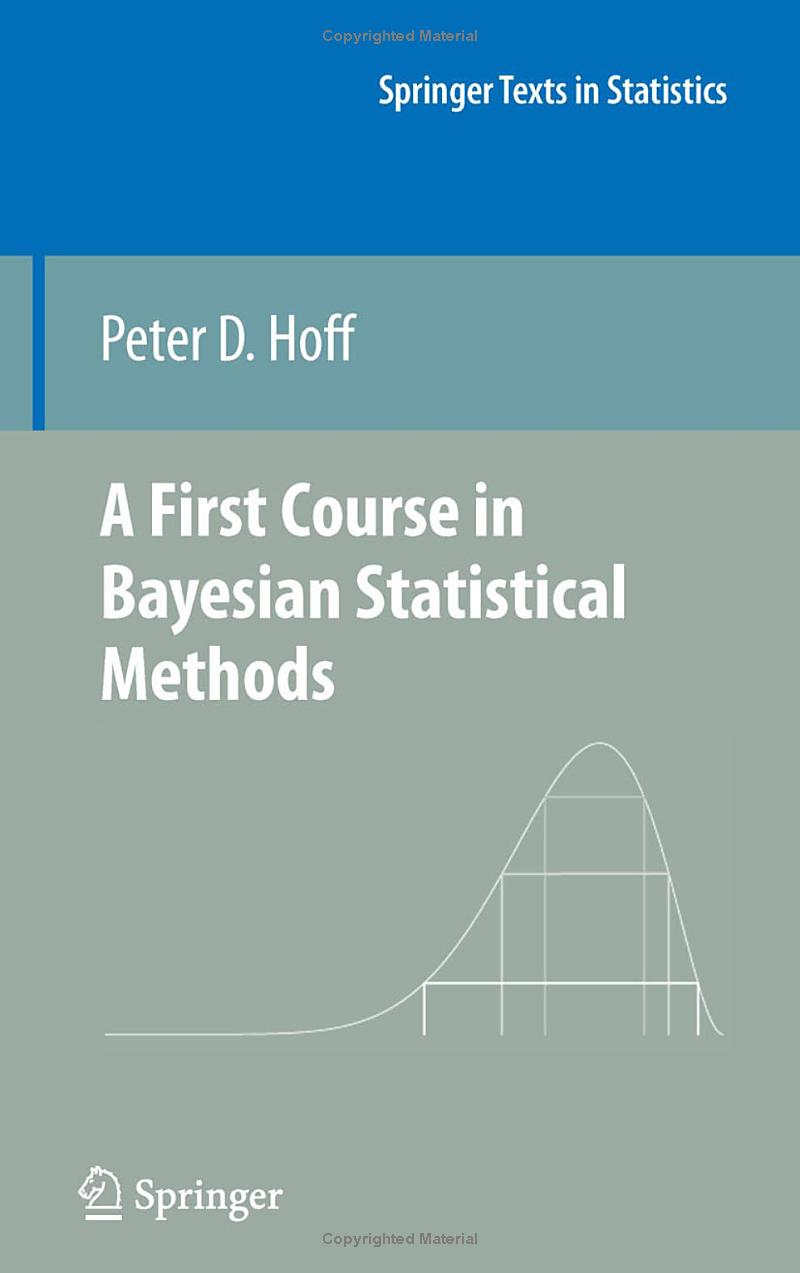
\includegraphics[height=.65\paperheight]{Figure/hoff_first_bayes_course}
\end{minipage}
~
\begin{minipage}{.48\textwidth}
\centering
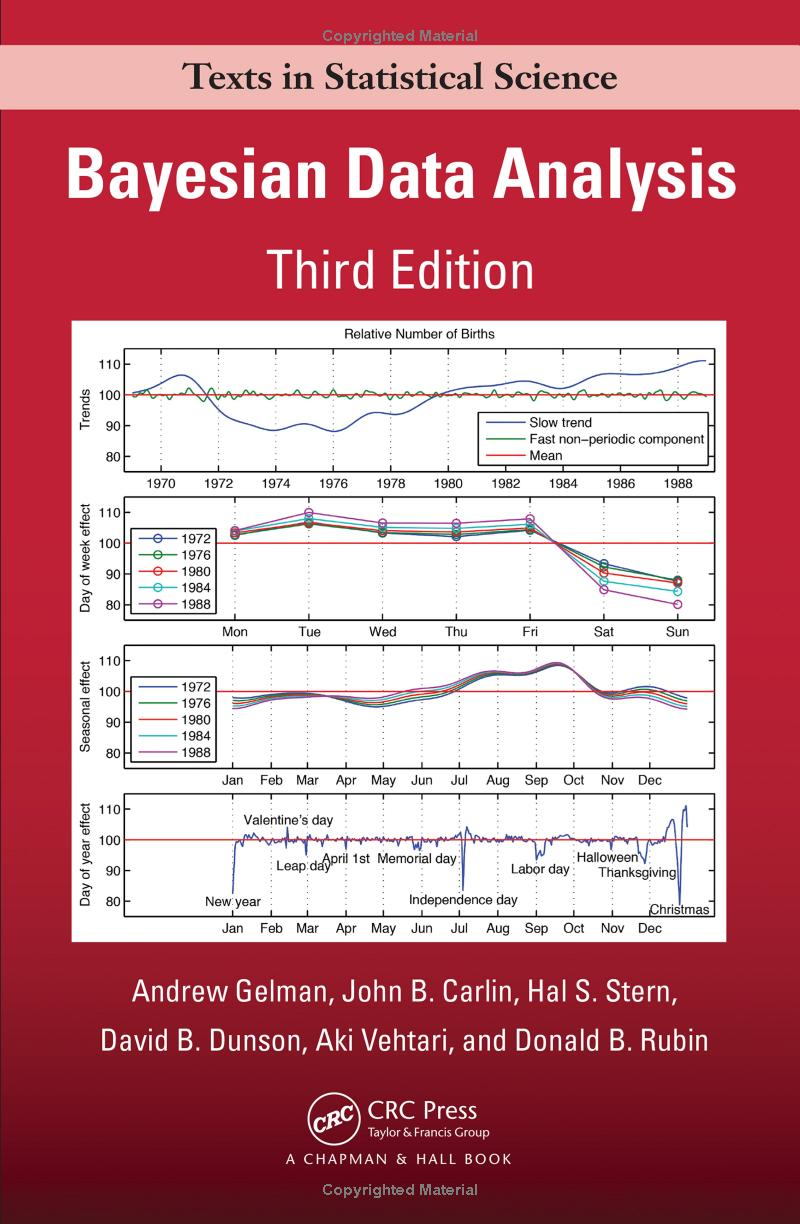
\includegraphics[height=.65\paperheight]{Figure/bda3}
\end{minipage}

\end{frame}


\begin{frame}
\frametitle{``Advanced introduction'' to Bayesian statistics}

\vspace*{-.5\baselineskip}
%Such courses usually assume an audience with little prior exposure to advanced (non-Bayesian) methods beyond intro statistics. \\
%Those courses spend a lot of time on basics and don't get very far:

Such courses usually assume little prior exposure beyond intro statistics, spend a lot of time on basics, and don't get very far:
 
{\centering

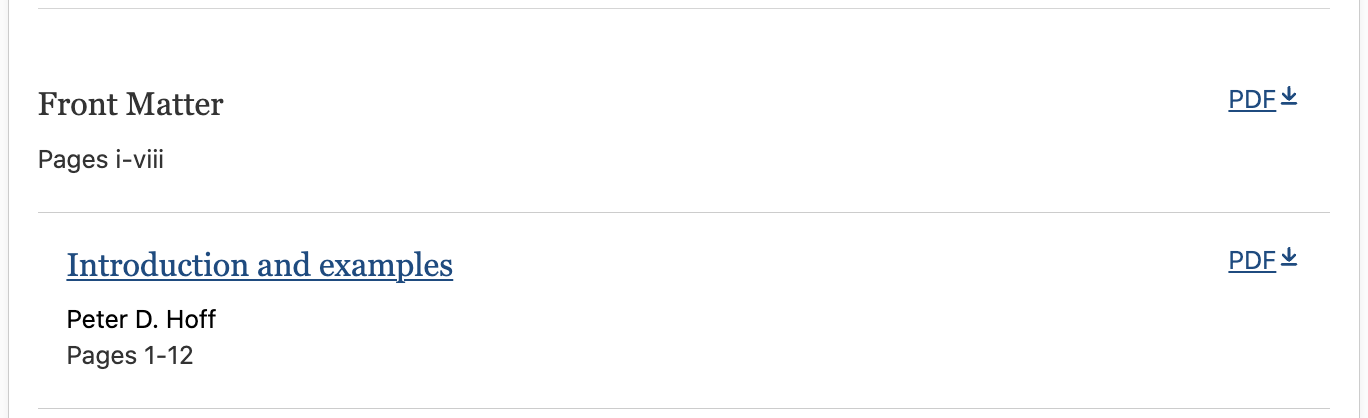
\includegraphics[width=.6\linewidth]{Figure/hoff_toc_head}

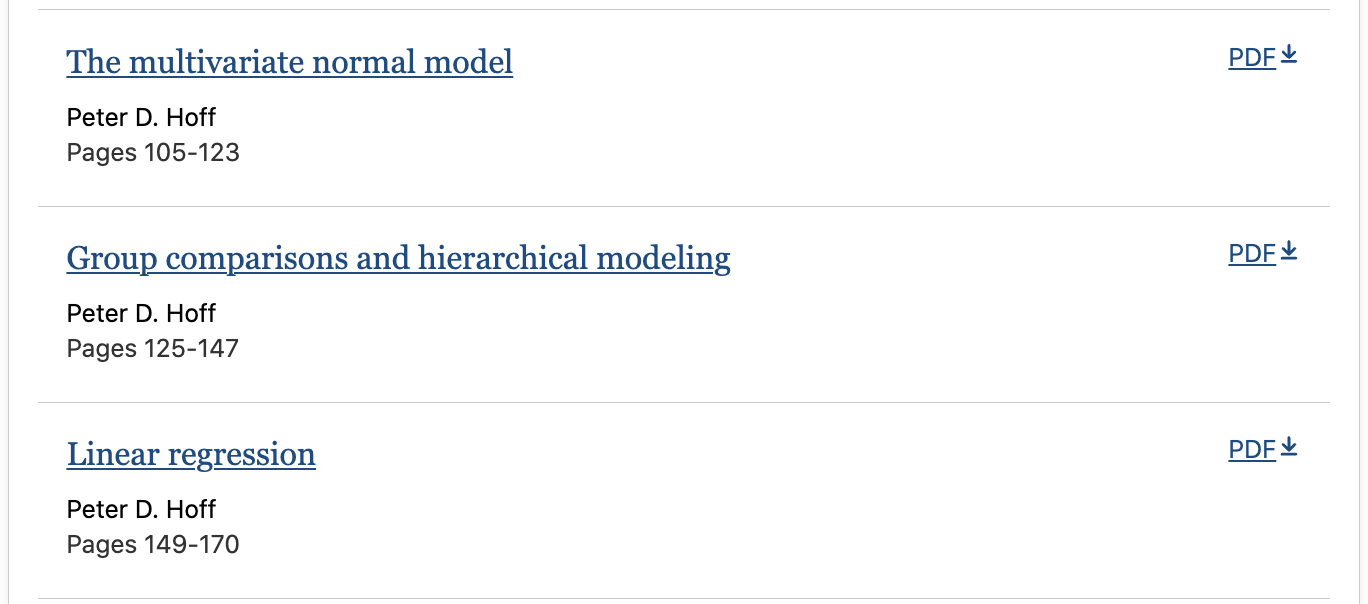
\includegraphics[width=.6\linewidth]{Figure/hoff_toc_middle}

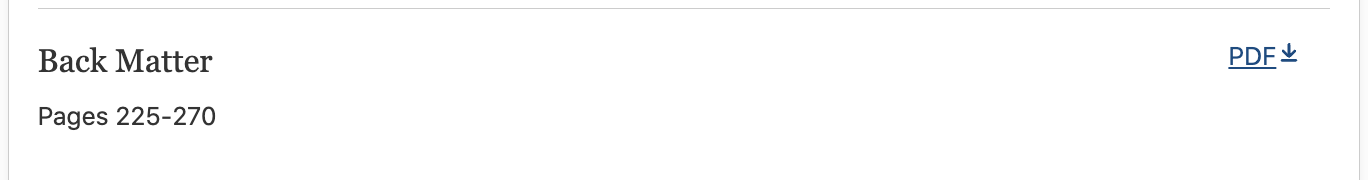
\includegraphics[width=.6\linewidth]{Figure/hoff_toc_foot}

}
\end{frame}


\begin{frame}
\frametitle{``Advanced introduction'' to Bayesian statistics}

{\centering

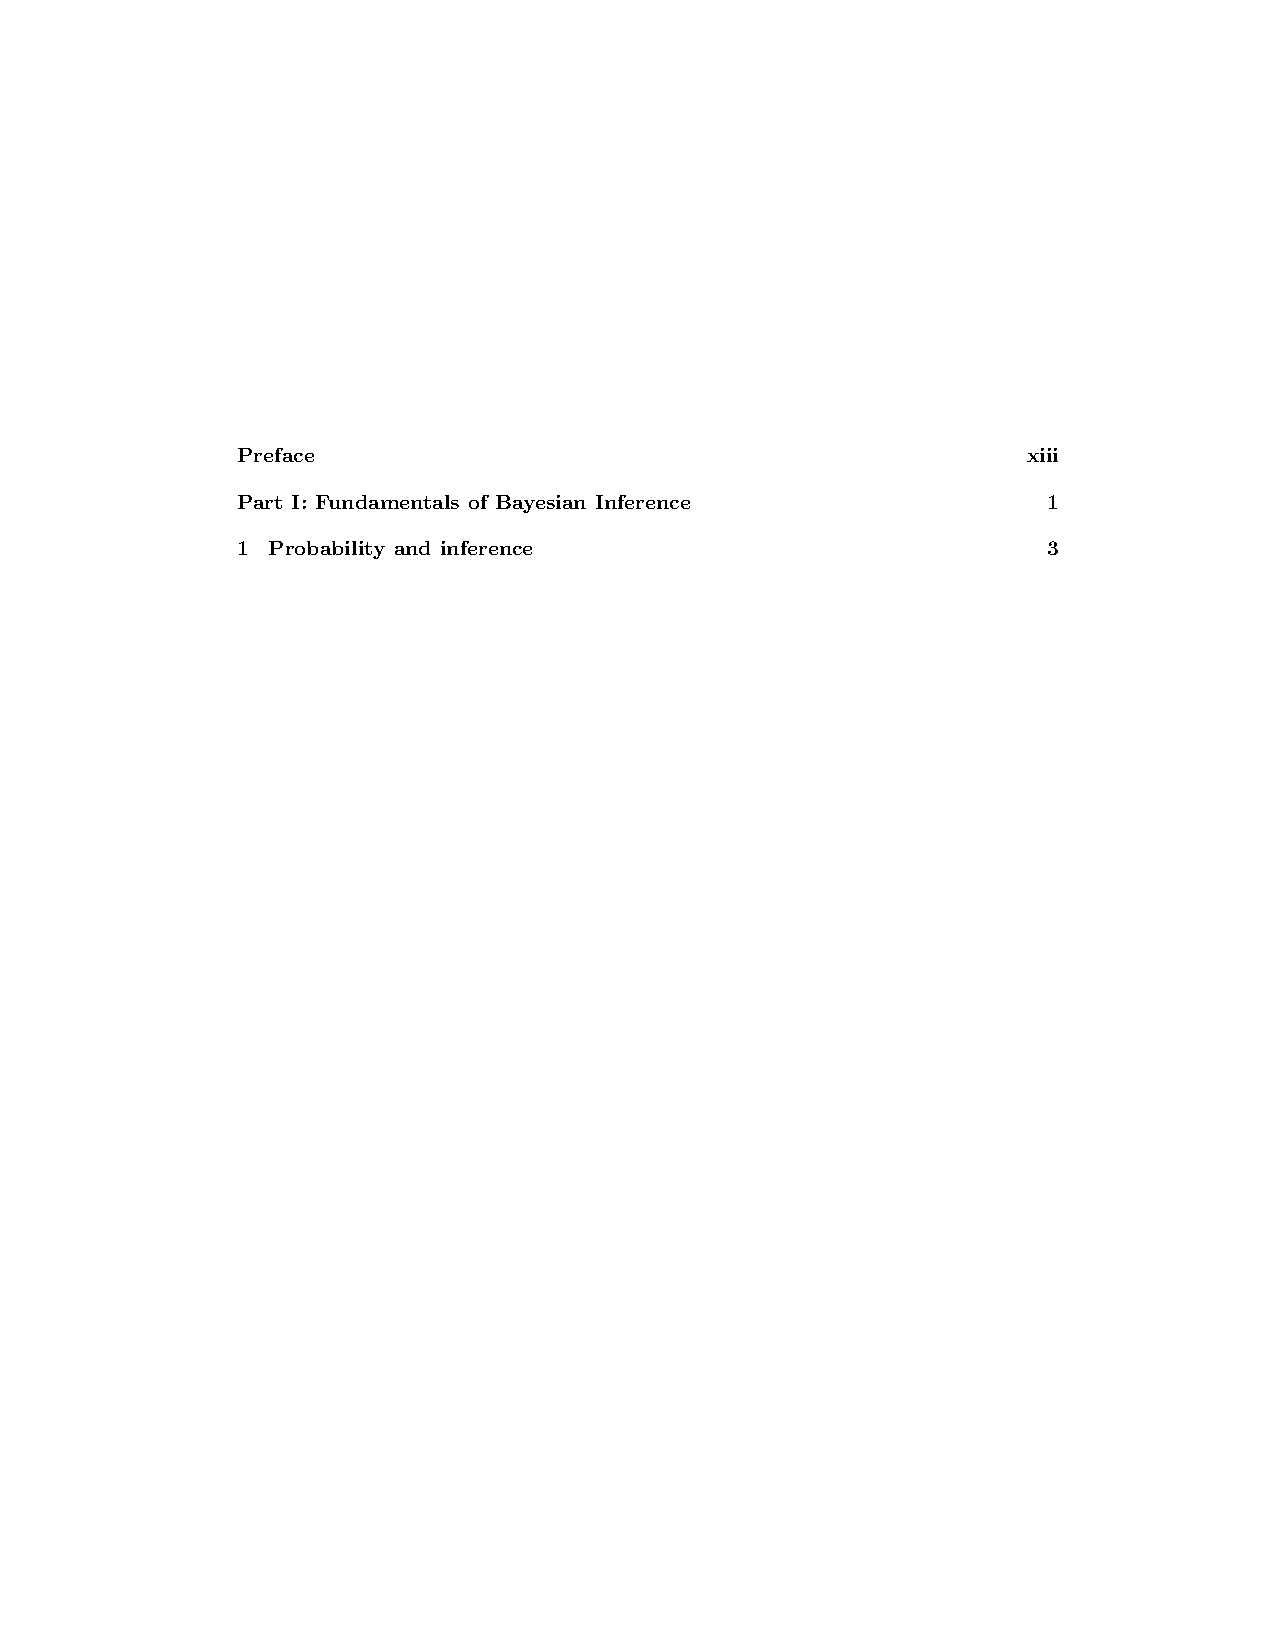
\includegraphics[width=.7\linewidth]{Figure/bda_toc_head}

\vspace*{-.8\baselineskip}
\scalebox{.5}{$\vdots$}
\vspace*{-.2\baselineskip}

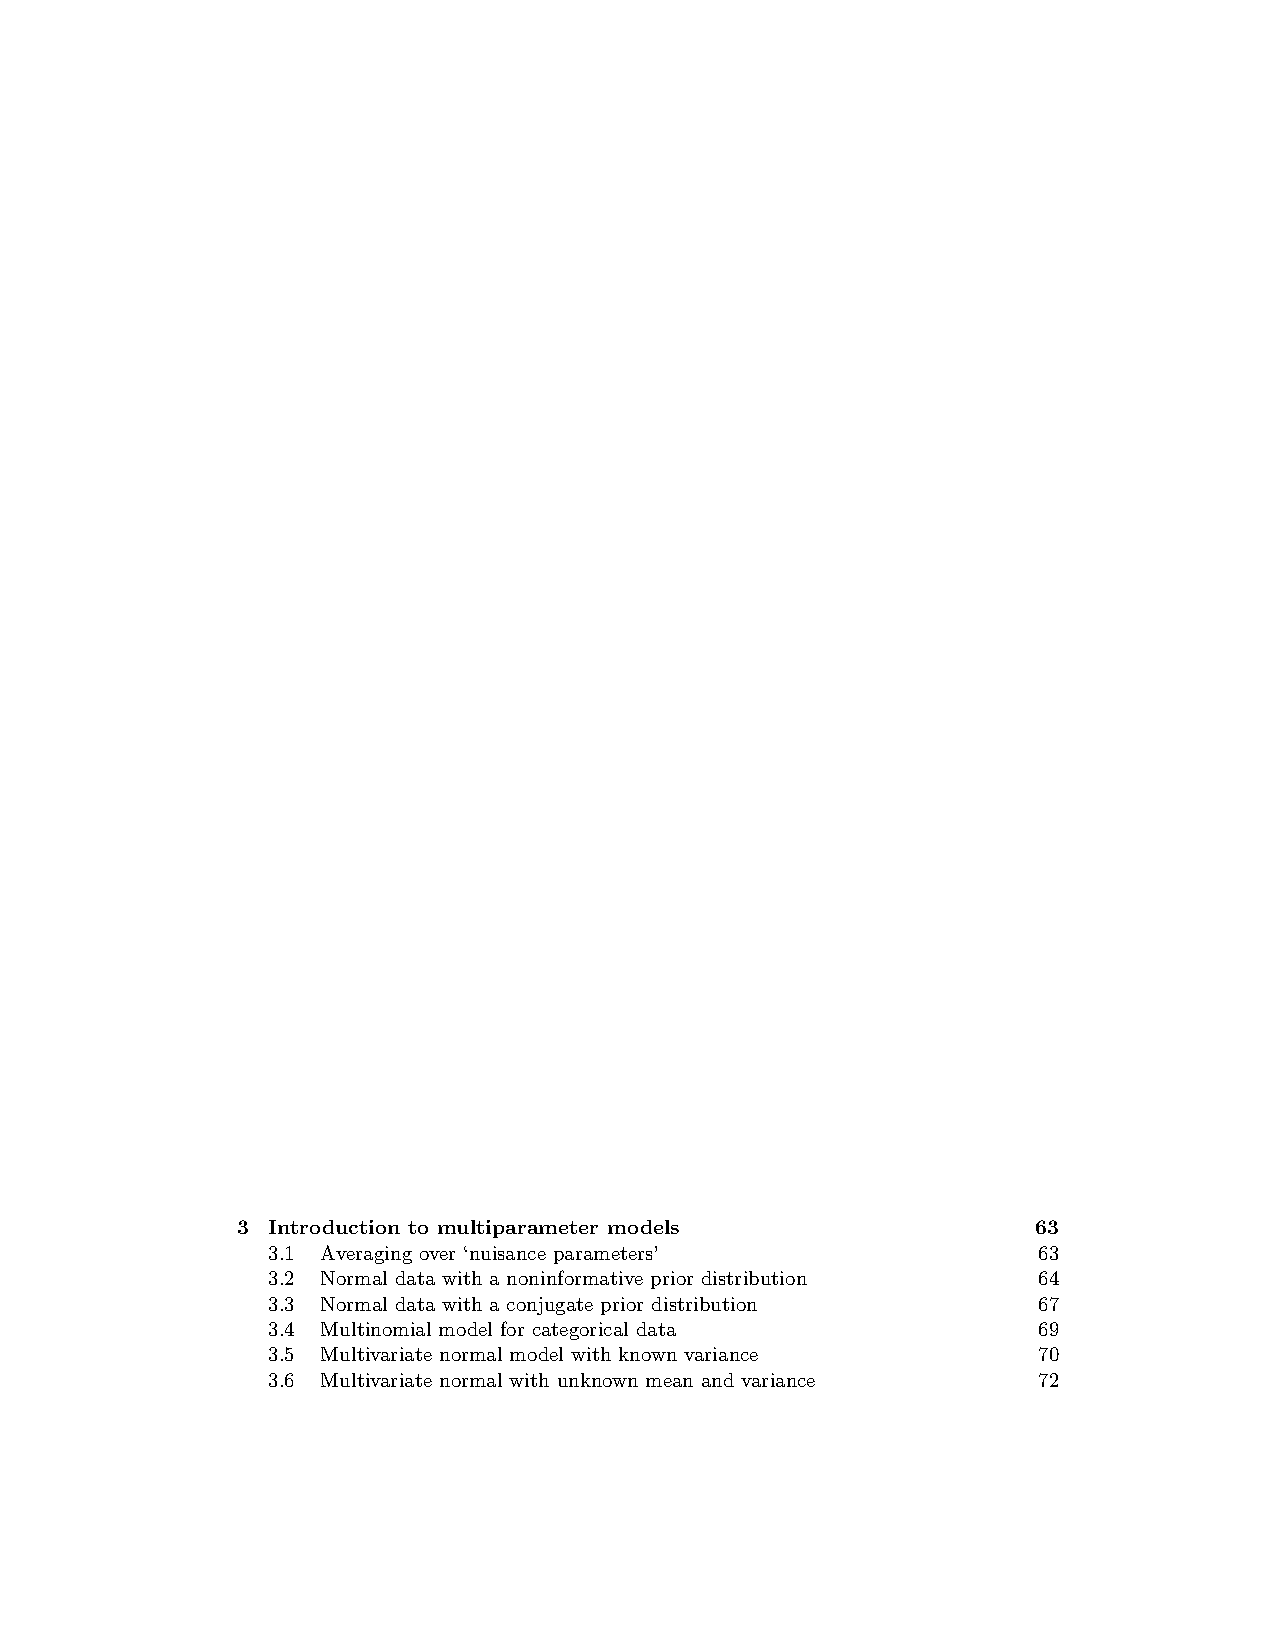
\includegraphics[width=.7\linewidth]{Figure/bda_toc_middle_1}

\vspace*{-.8\baselineskip}
\scalebox{.5}{$\vdots$}
\vspace*{-.2\baselineskip}

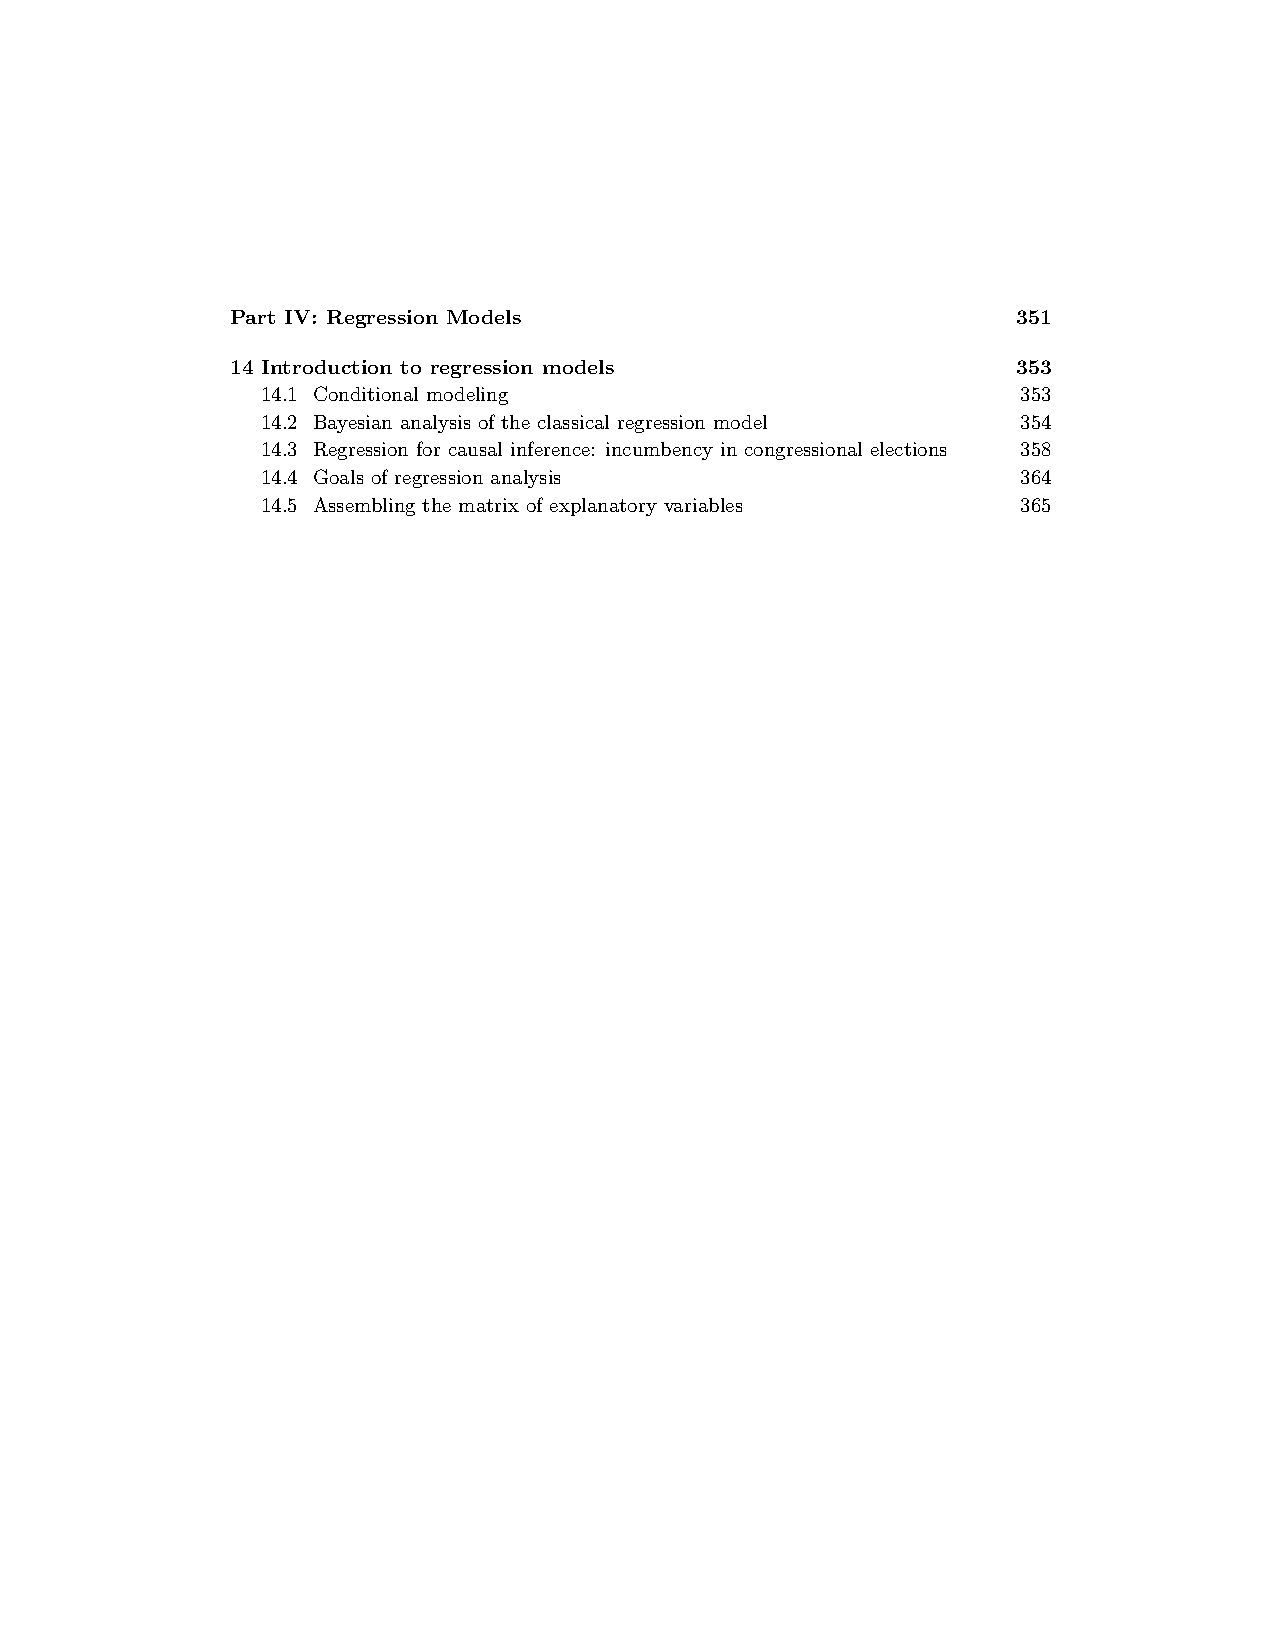
\includegraphics[width=.7\linewidth]{Figure/bda_toc_middle_2}

\vspace*{-.8\baselineskip}
\scalebox{.5}{$\vdots$}
\vspace*{-.2\baselineskip}

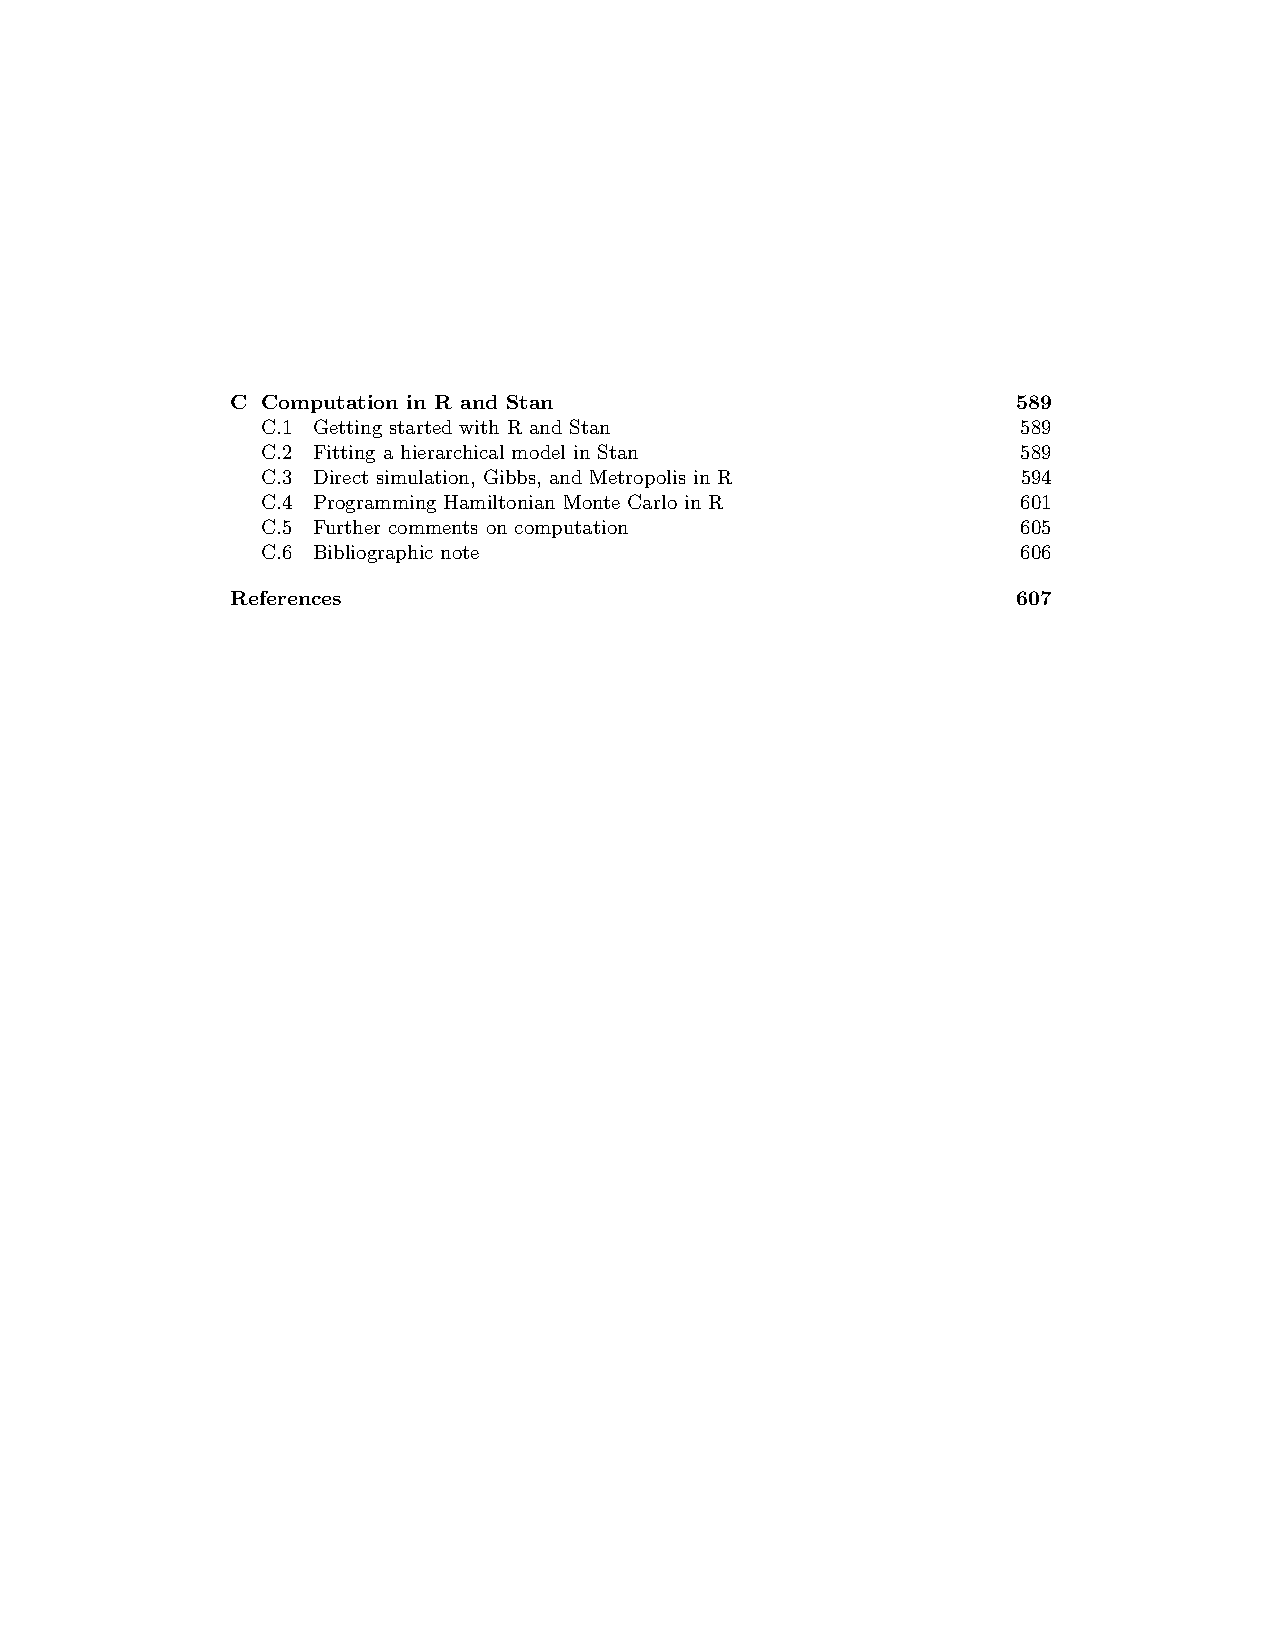
\includegraphics[width=.7\linewidth]{Figure/bda_toc_foot}

}
%Shortcoming of such courses is their Bayes-centric assumptions:
%\begin{itemize}
%\item Students' first exposure to 
%\item 
%\end{itemize}

\end{frame}


\begin{frame}
\frametitle{``Advanced introduction'' to Bayesian statistics}

{\fontdimen2\font=.7ex 
This is unfortunate b/c Bayes in basic settings give mostly the same answers as their freq counterparts and doesn't offer much beyond.} 
% Note: Starting with basics would makes sense if we lived a world where students learn statistics primarily through Bayes lens, but we don't.

\pause
\smallskip
Worse, only teaching Bayesian approaches to problems that have perfectly fine existing solutions seems to risk promoting fanaticism:

\begin{center}
\begin{minipage}{.93\linewidth}
{\slshape
``Everyone uses Bayesian inference when it is clearly appropriate. A Bayesian is someone who uses Bayesian inference even when it might seem inappropriate.''}

\hfill \citep{gelman2013bayes_absurdity}
\end{minipage}
\end{center}

\end{frame}


\begin{frame}
\frametitle{``Advanced introduction'' to Bayesian statistics}

This ain't good when the legacy of Great Bayes-Frequentist War lingers to this day:

\begin{center}
\begin{minipage}{.87\linewidth}
{\slshape
``The missionary zeal of many Bayesians of old has been matched, in the other direction, by an attitude among some theoreticians that Bayesian methods were absurd—not merely misguided but obviously wrong in principle.'}

\vspace*{.3\baselineskip}
\hfill \citep{gelman2013bayes_absurdity}
\end{minipage}
\end{center}

\end{frame}


\begin{frame}
\frametitle{``Advanced introduction'' to Bayesian statistics}

It also gives students a wrong impression that Bayes is about priors which, besides being incorrect, has caused Bayes some bad rap:

\begin{center}
\begin{minipage}{.89\linewidth}
{\slshape
One misconception (of many) about Bayesian analyses is that prior distributions introduce assumptions that are more questionable than assumptions made by frequentist methods; yet the assumptions in priors can be more reasonable than the assumptions implicit in standard frequentist models.}

\vspace*{.3\baselineskip}
\hfill \citep{greenland2006bayes_for_epi}
\end{minipage}
\end{center}

\end{frame}


\begin{frame}
\frametitle{``Advanced introduction'' to Bayesian statistics}

{\fontdimen2\font=.65ex 
This ``advanced intro'' is my attempt, within the practical constraits, 
}%
to address the drawbacks of the traditional intro to Bayes.

\pause
\textbf{Features:} 
\begin{tightItemize}[<+->]
\item Proceeds more quickly through standard models, assuming substantial familiarity with (non-Bayesian) statistical inference;
\item Explores, whenever practically relevant, similarities and differences between Bayes and freq approaches;
\item Prioritizes foundational principles over applied modeling.
	% Note: Though this is not to say that the course isn't important for applied Bayesian modellers. 
\end{tightItemize}

\end{frame}


\begin{frame}
\frametitle{Who is this course for?}

I imagine you are interested in this course because you want to become, broadly speaking, one (or more) of the following kinds: 

\vspace*{.5\baselineskip}
\begin{indented}
Casual Bayes users\\ \vspace*{-.4\baselineskip}

\begin{indented}
\only<2->{who rely mainly on non-Bayesian techniques but take occasional inspirations from Bayes when advantageous to do so.}
% Note: frequentist properties of Bayes, Bayesian occam's razor, complexity-adaptive ability of Bayes for complex ML models
\end{indented} 

Applied Bayesian modelers\\ \vspace*{-.4\baselineskip}

\begin{indented}
\only<3->{%
who leverage the flexibility of Bayes to account for complex \\
scientific and hierarchical structures in their applied research.
}%
% Note: Knowing mechanics of Bayesian inference helps troubleshoot issues when they arise. Behavior of Bayesian procedures are very different from frequentist onces but, once you understand it, they tend to be more intuitive.
\end{indented}

Bayes enthusiasts/experts\\ \vspace*{-.9\baselineskip}

\begin{indented}
\only<4>{who pursue advancing Bayesian methods in their research.}

% Note: Comment on how to supplement the knowledge from this course with further (self-)studies.
\end{indented}

\end{indented}

\end{frame}


\section{\centerline{What's Bayesian statistics about?}}


\begin{frame}
\frametitle{Meet Bayes' rule}

Bayesian analysis starts by assigning a probabilistic model to observed $\by$, yielding \textit{likelihood} $\likelihood(\by \given \btheta)$ parametrized by unknown $\btheta$.

\pause
\smallskip
It then places a \textit{prior} dist $\density(\btheta)$ on the parameter to be estimated.

\pause
\smallskip
Conceptually, this is all that's required; 
basic math then tells us, having observed $\by$, the \textit{posterior} dist on unknown $\btheta$ is given by
\begin{equation*} \defineTightSpacing%
\density(\btheta \given \by) 
	\propto \likelihood(\by \given \btheta) \thinnerspace \density(\btheta).
\end{equation*}
\pause%
This \textit{Bayes' rule} follows from the fact $\thinnerspace \density(\btheta \given \by) \thinnerspace \likelihood(\by) = \likelihood(\by \given \btheta) \thinnerspace \density(\btheta)$.

\pause
\smallskip
\mbox{\textbf{Note:} Notation $f(\btheta, \bm{\phi}, \by) \negthinnerspace \propto \negthinnerspace g(\btheta)$ means $f(\btheta, \bm{\phi}, \by) \negthinnerspace = \negthinnerspace C(\bm{\phi}, \by) \thinnerspace g(\btheta)$}
and is used b/c we often need densities known only up to constant.

\end{frame}


\begin{frame}
\frametitle{Example: Bayesian latent var.\ model}

Power of Bayes lies in its ability to accommodate elaborate $\likelihood(\by \given \btheta)$:

\pause
\begin{figure}
\centering
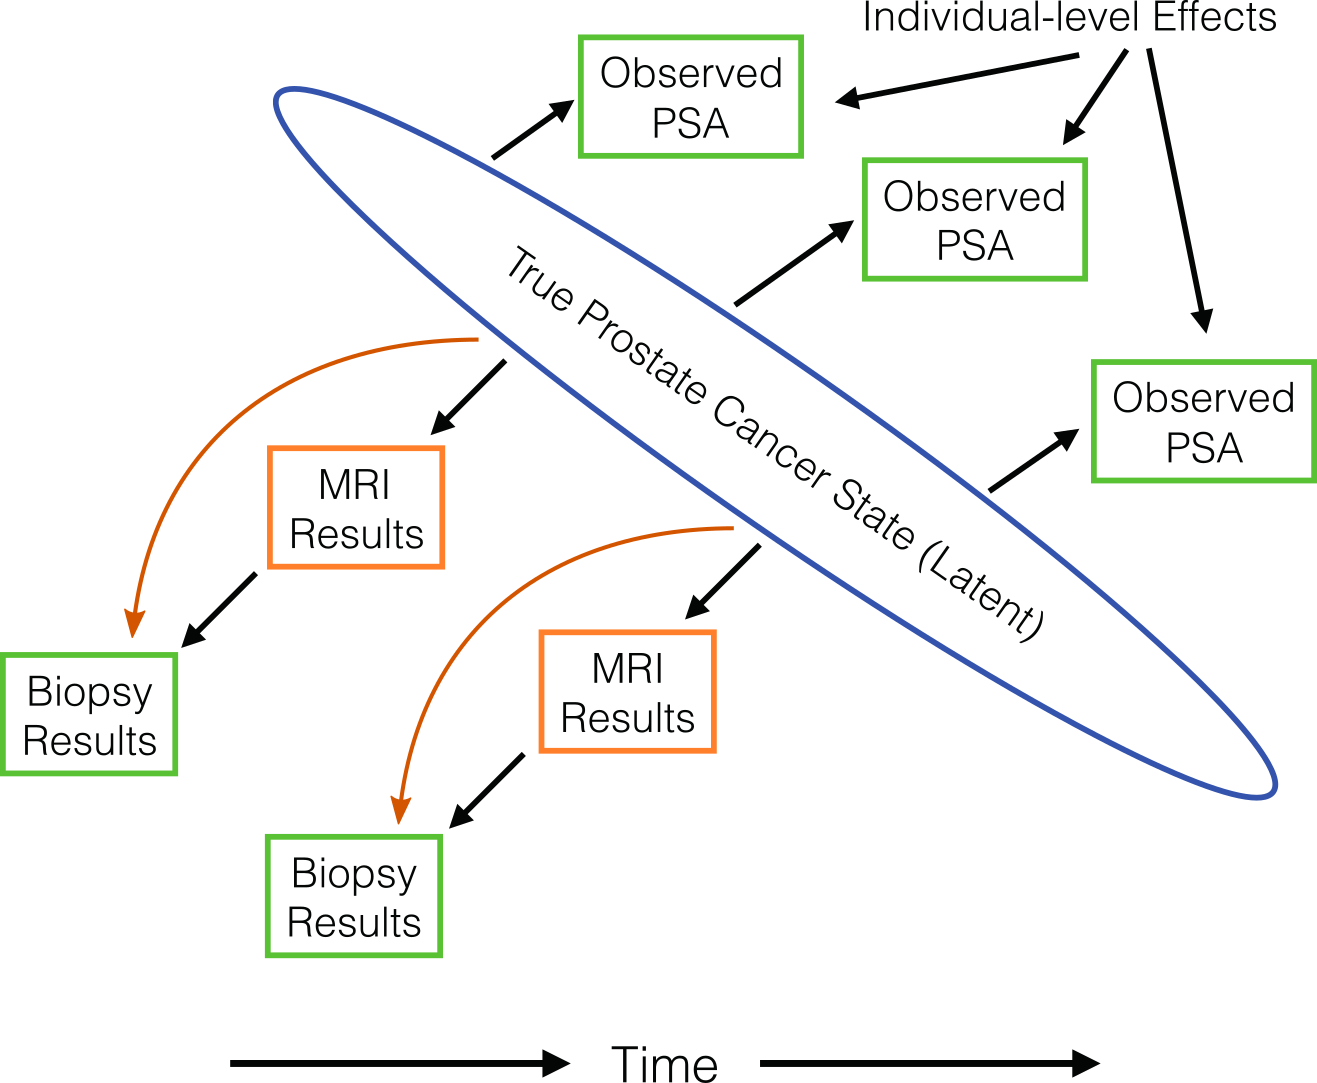
\includegraphics[width=.6\linewidth]{Figure/active_surveillence_model_with_mri}

\vspace*{.1\baselineskip}
\caption*{\textcolor{themecolor}{\textbf{Figure:}}
	Surveilance of prostate cancer through surrogate measures.%
}%
\end{figure}

\end{frame}


\begin{frame}
\frametitle{Example: Bayesian \textcolor{jhuSpiritBlue}{hierarchical} latent var.\ model}

\begin{figure}
\centering
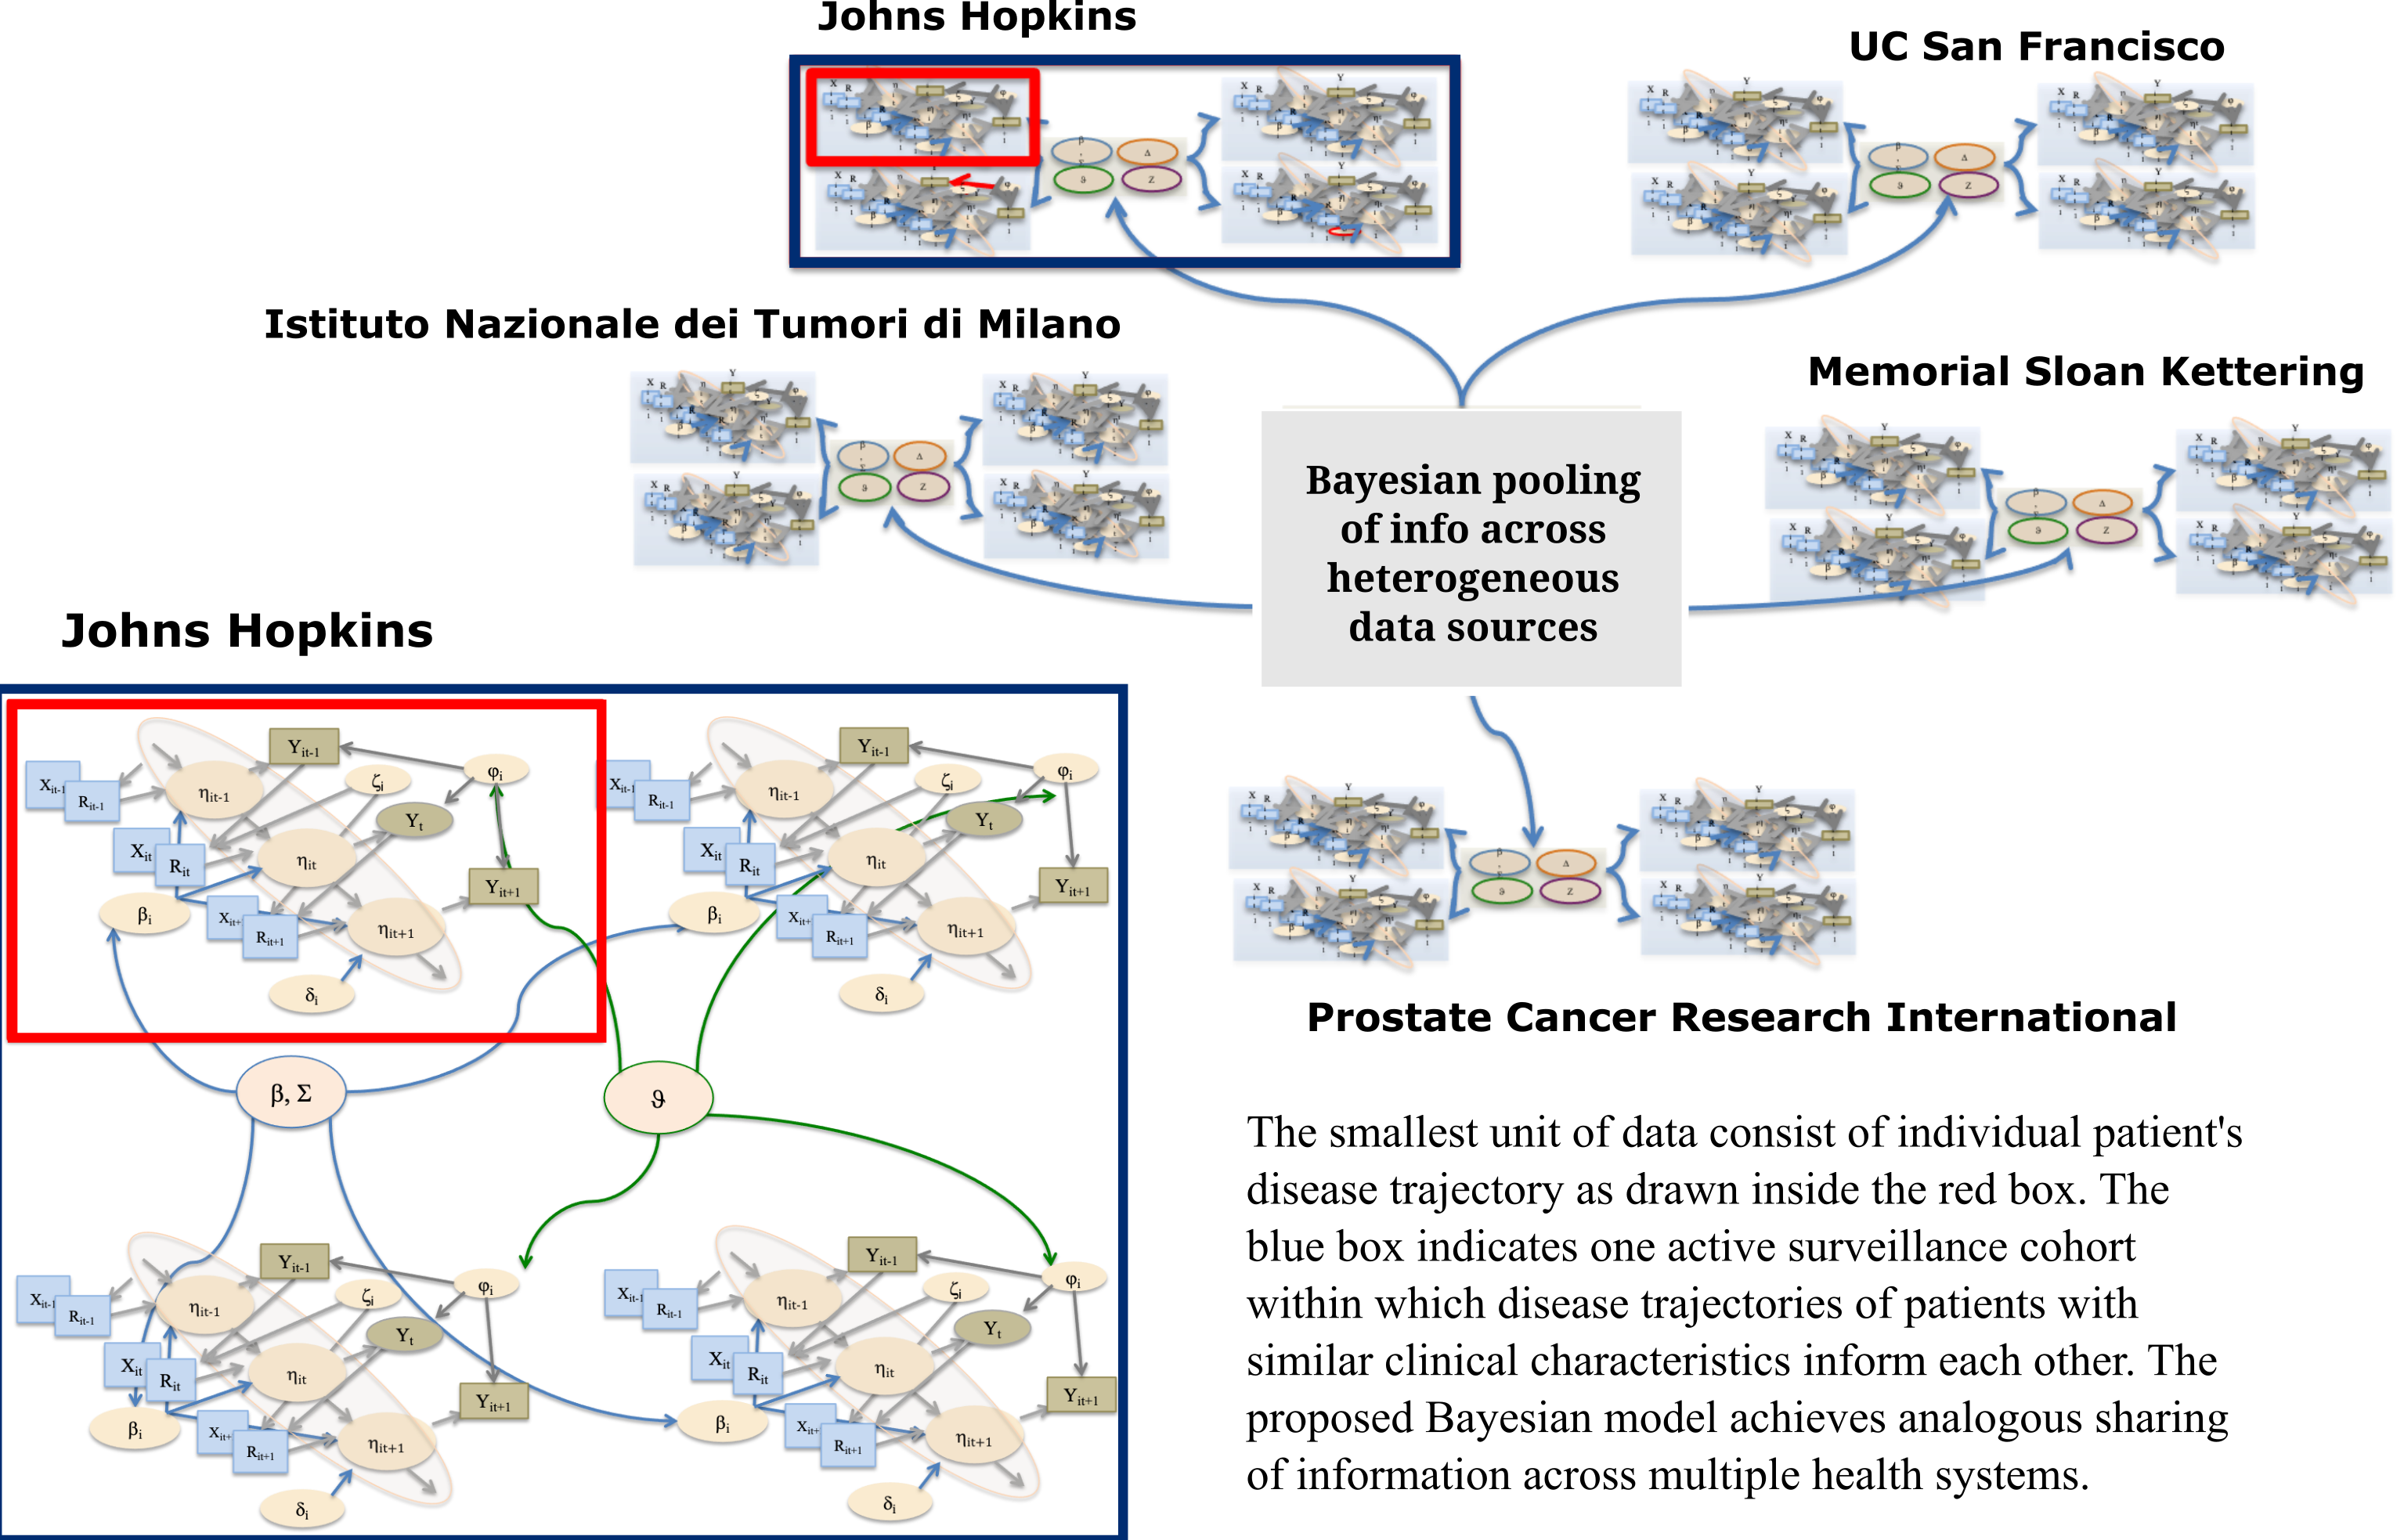
\includegraphics[width=\linewidth]{Figure/bayesian_hierarchical_modeling_of_multiple_cohorts}
\end{figure}

\end{frame}


\begin{frame}
\frametitle{Example:  \st{Bayesian} Probabilistic topic model}
\vspace*{.15\baselineskip}

\hspace*{-.03\linewidth}
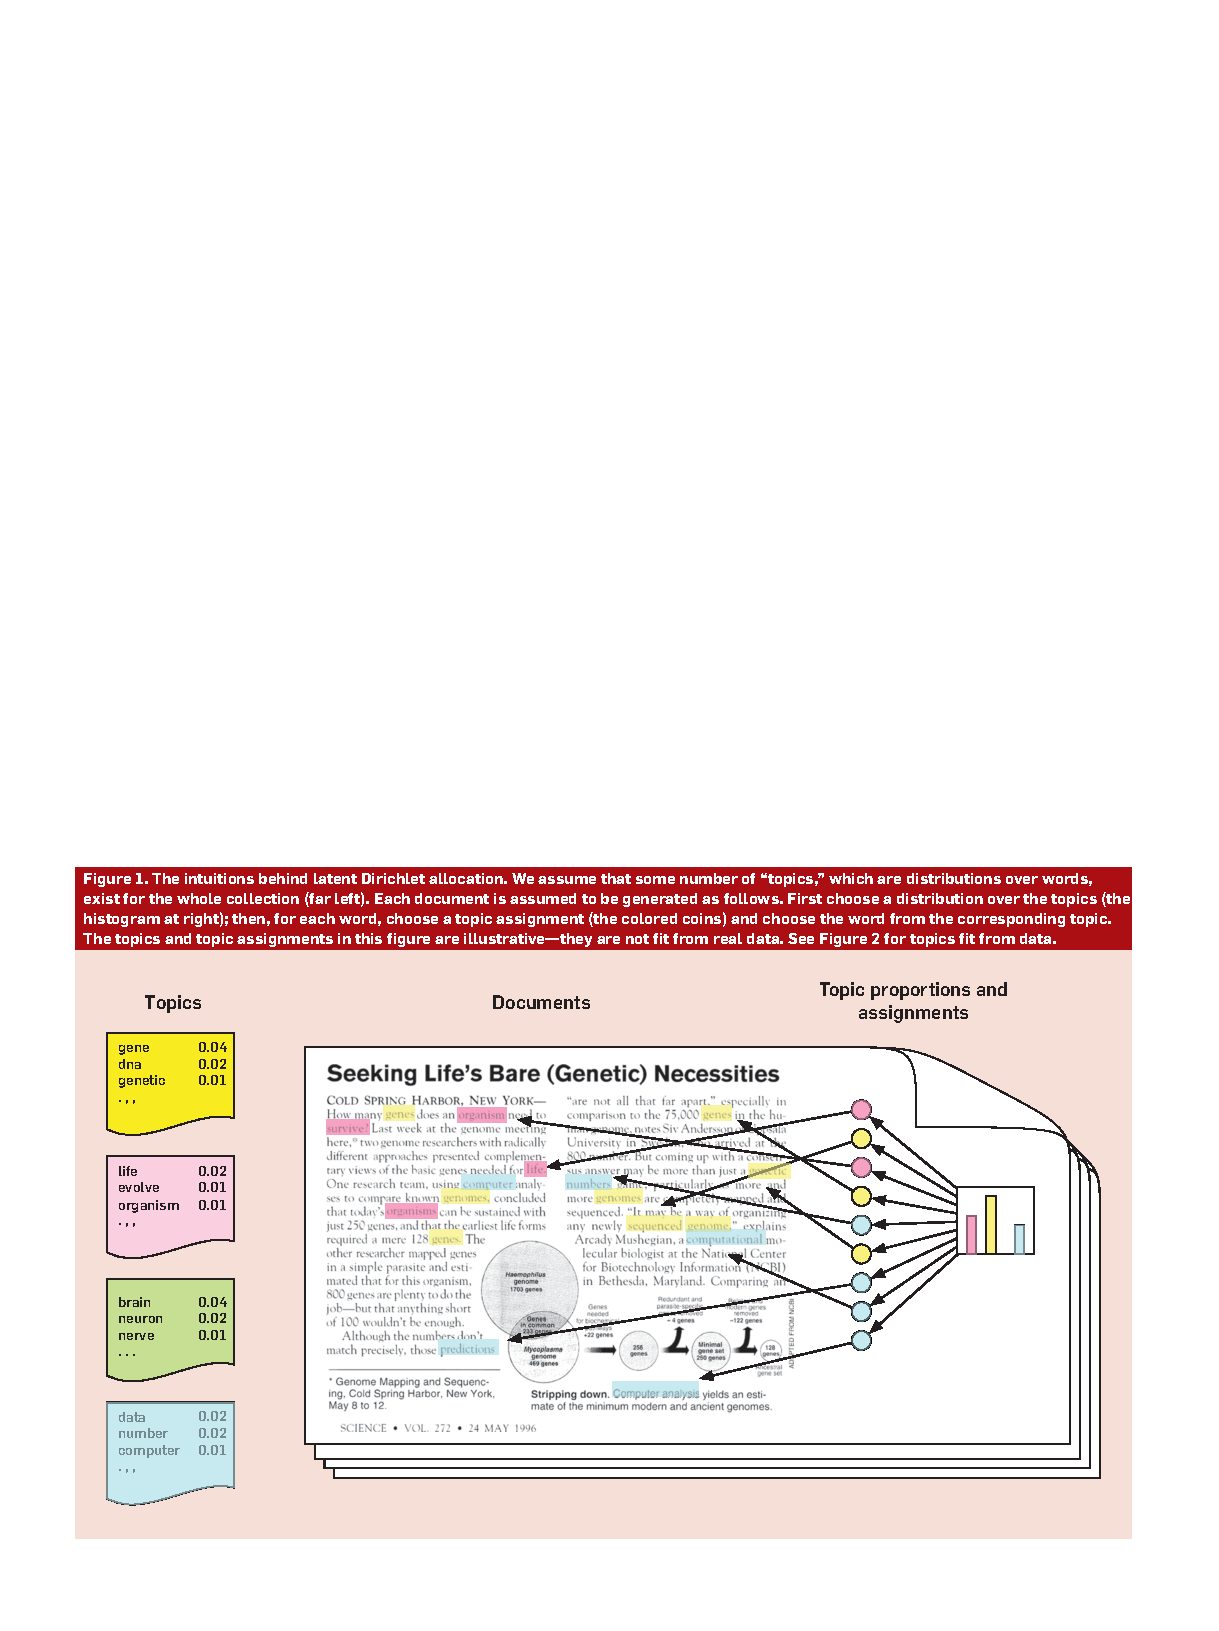
\includegraphics[width=1.04\linewidth]{Figure/lda_viz}
\end{frame}


\begin{frame}
\frametitle{Example:  \st{Bayesian} Probabilistic topic model}
\vspace*{.15\baselineskip}

\hspace*{-.03\linewidth}
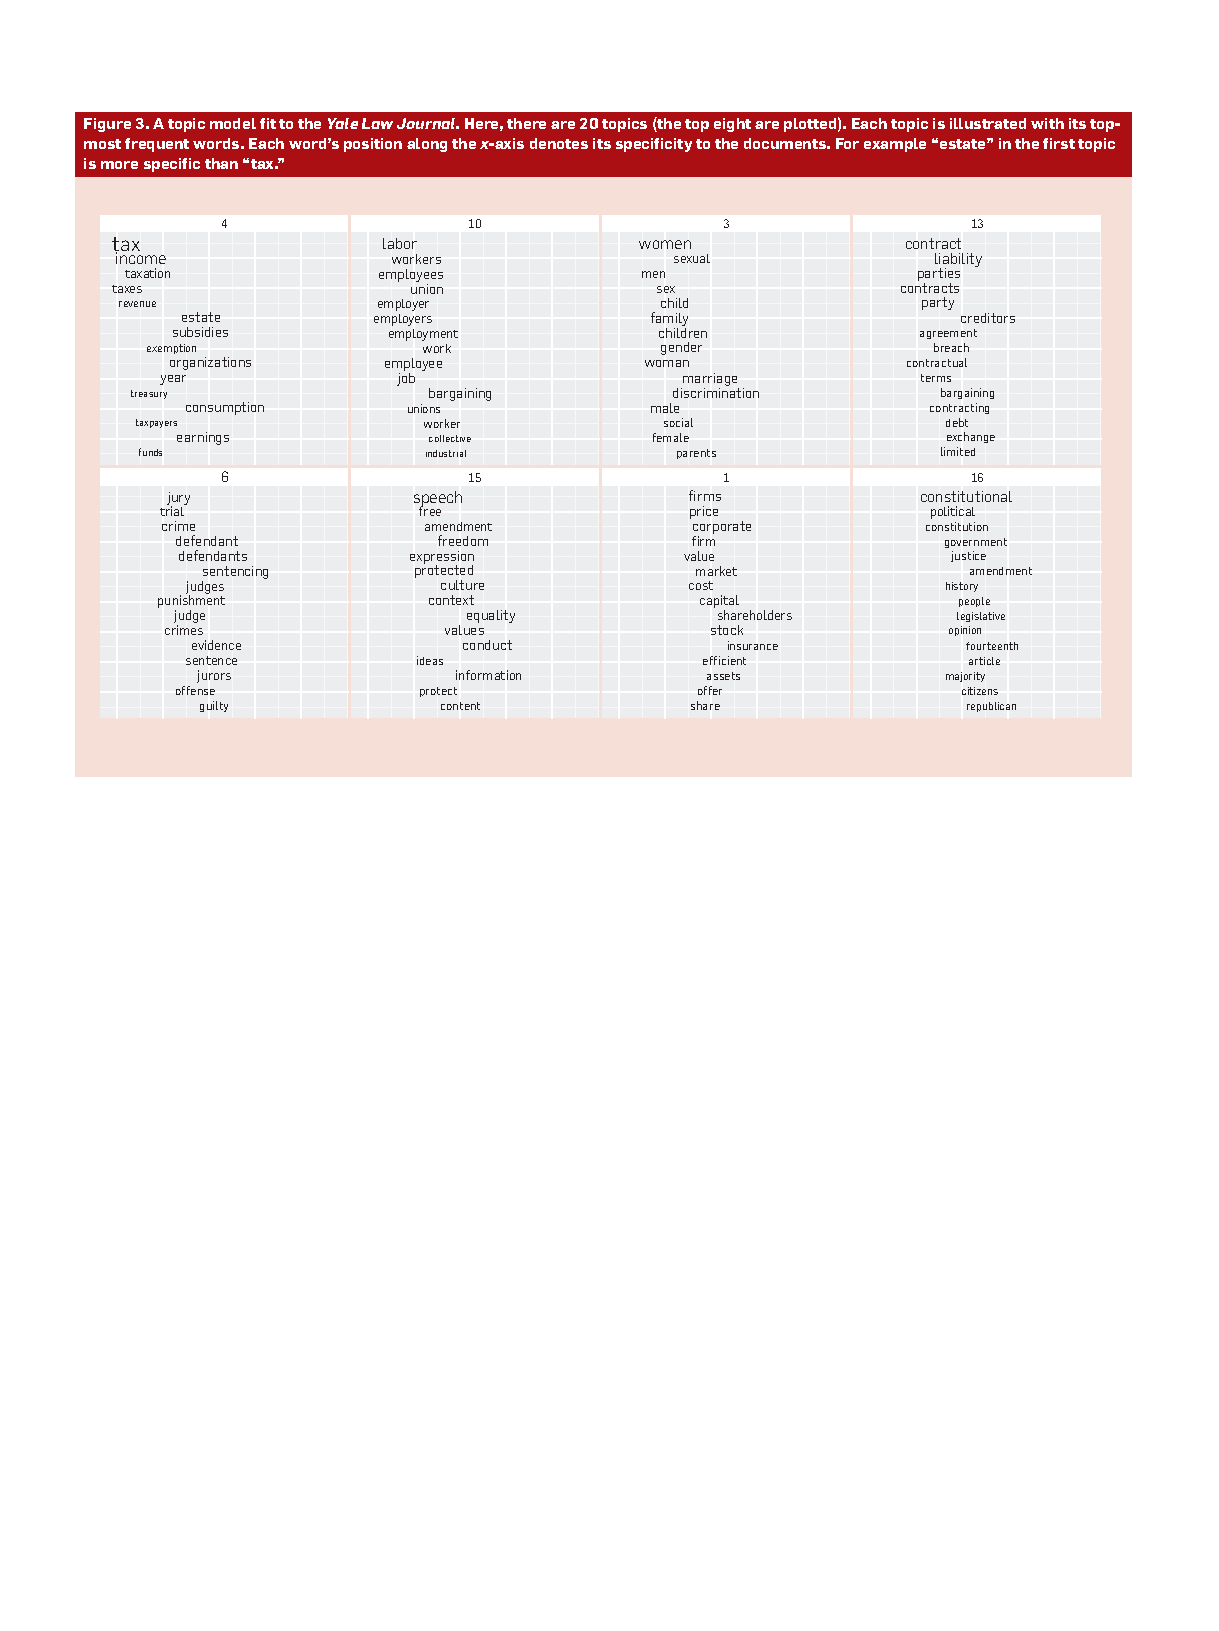
\includegraphics[width=1.04\linewidth]{Figure/lda_on_law_journal}
\end{frame}


\begin{frame}
\frametitle{Example:  \st{Bayesian} Probabilistic topic model}
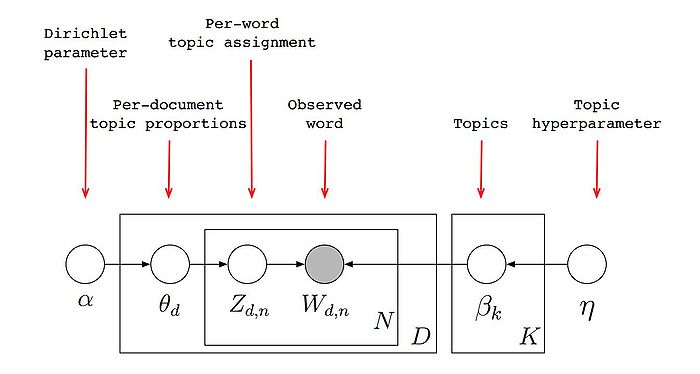
\includegraphics[width=\linewidth]{Figure/lda_dag}
% Source: https://github.com/SoojungHong/TextMining/wiki/LDA-and-Topic-Modeling
\end{frame}


\begin{frame}
\frametitle{Statistics in post Bayes-Frequentist War era}

\includegraphics[width=\linewidth]{Figure/why_isnt_everyone_bayesian_top}
\vspace*{-.9\baselineskip}%

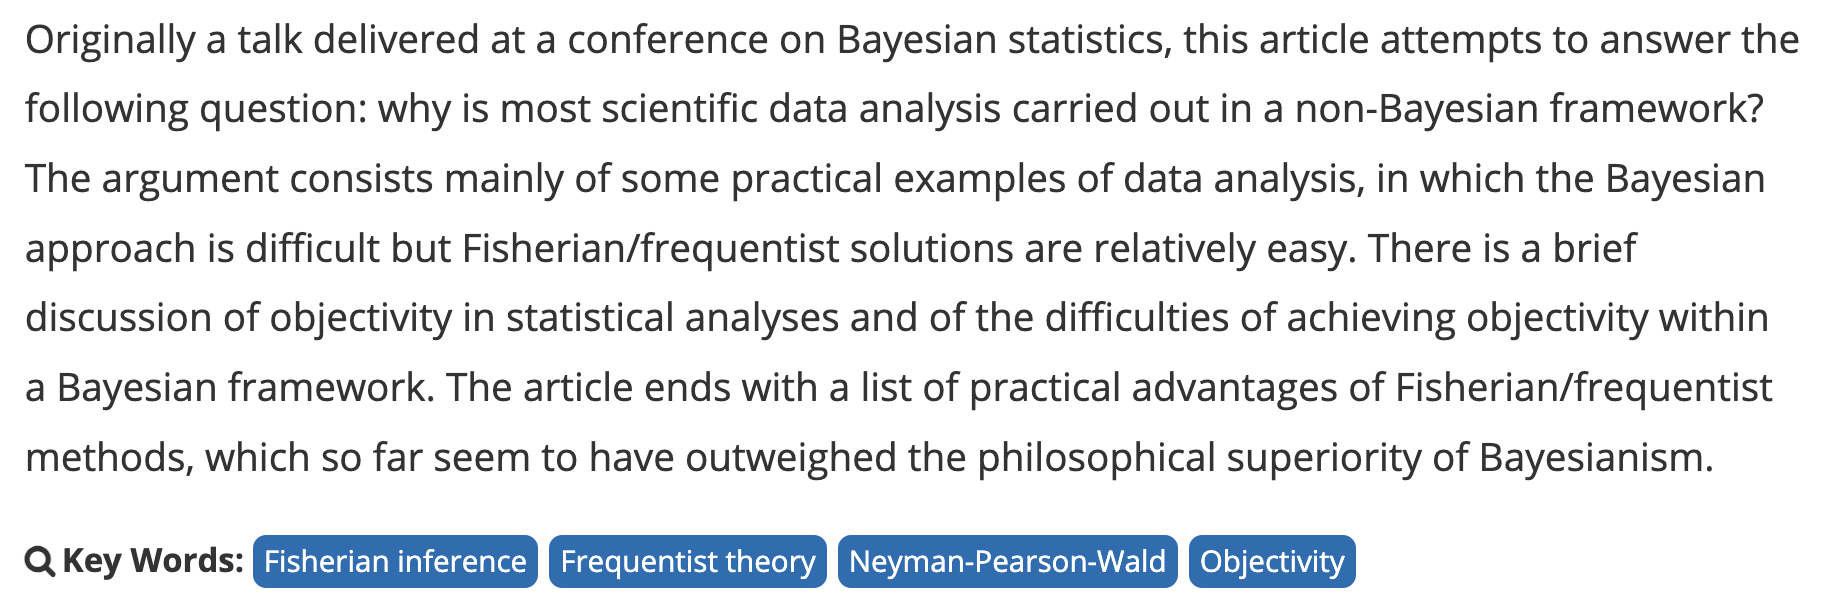
\includegraphics[width=\linewidth]{Figure/why_isnt_everyone_bayesian_bottom}
\end{frame}


\begin{frame}
\frametitle{Statistics in post Bayes-Frequentist War era}
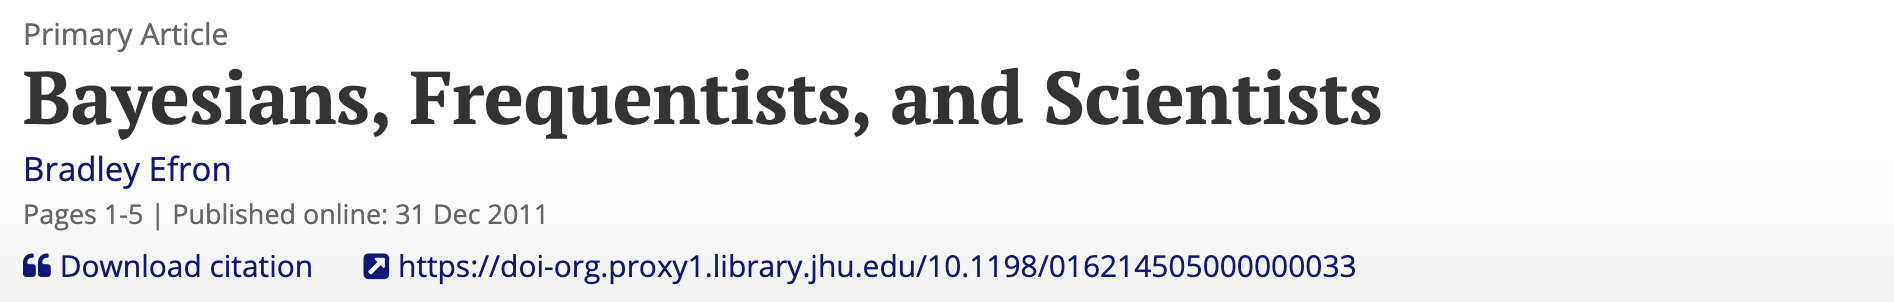
\includegraphics[width=\linewidth]{Figure/bayes_freq_scientist_top}
\vspace*{-.9\baselineskip}%

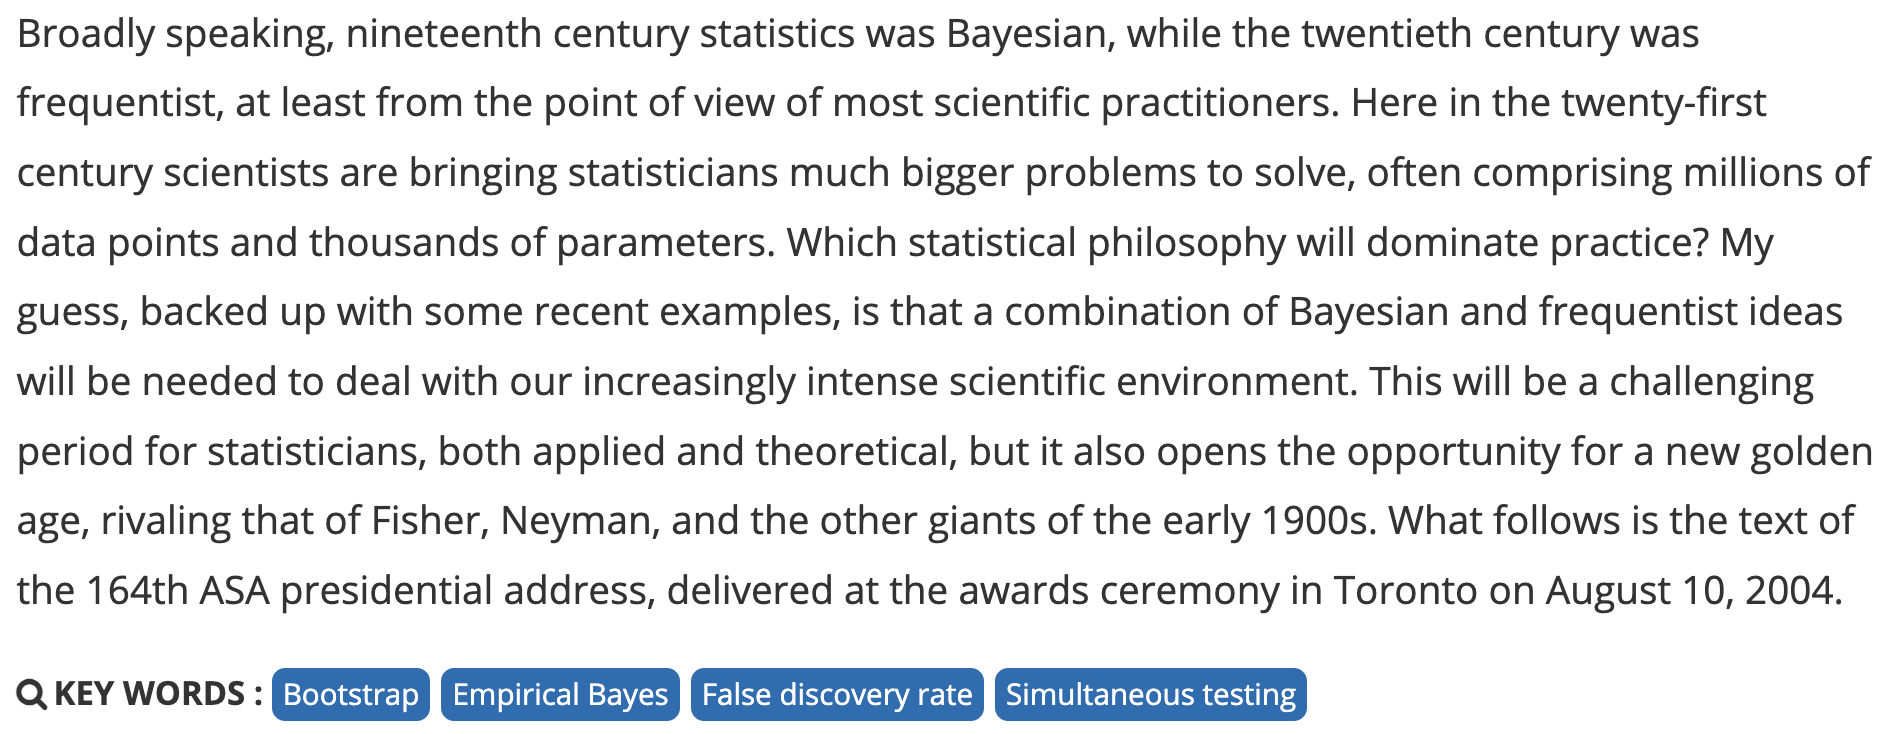
\includegraphics[width=\linewidth]{Figure/bayes_freq_scientist_bottom}
\end{frame}

\nobibliography{references} % To cite inline without creating a bibliography
\end{document}